
 \section{Task}

 \begin{figure}[h!]
 \centering
 
\includegraphics[width=0.3\textwidth]{./Pictures/ARIS_logo.png}
 \caption{Official logo of ARIS \cite{ARIS}}
 \label{fig:ArisLogo}
\end{figure}

 The Academic Space Initiative Switzerland (ARIS) is a student association which competes in the yearly Intercollegiate Rocket Engineering Competition (IREC).
 The goal of this competition is to build a rocket that can fly autonomously to a predefined apogee (10 000 feets = 3048 meters) and after that return safely back to the ground with the help of parachutes.
 Additionaly the rocket has to be able to transport a specific amount of payload with it.
 There are a total of 1 000 points to achieve in the competition which are based on different parts depicted in Table \ref{tab:CompetitionCalculation}.

\begin{table}[h]
\centering
\begin{tabular}{|l|l|l|}\hline
{\bf Description} & {\bf Points} & {\bf Percent}\\\hline
Entry form and progress update & 60 & 6 \% \\ \hline
Technical report & 200 & 20 \% \\ \hline
Design implementation & 240 & 24 \% \\ \hline
Flight performance & 500 & 50 \% \\ \hline
{\bf Total} & {\bf 1000} & {\bf 100} \% \\ \hline
\end{tabular}
\caption{Calculation of the points of the IREC}
\label{tab:CompetitionCalculation}
\end{table}


 It can be seen that just halve of the points are assigned to the performance at the competition itself.
 The other halve of the points can be achieved by teamwork, professional documentation and good engineering during the development and construction of the rocket.
 For the 500 points which are assigned to the flight performance, 350 are based on the error made between the targeted and approached apogee.
 These points are calculated like this:

 $$ Points =  350 - \frac{350}{0.3\cdot TargetedApogee} \cdot |TargetedApogee - ApproachedApogee|$$

 So there is a total of one point loss per 2.6 meters of deviation from the targeted apogee \cite{SpaceportAmericaCup2018}. \\

 \begin{figure}[h]
 \centering
 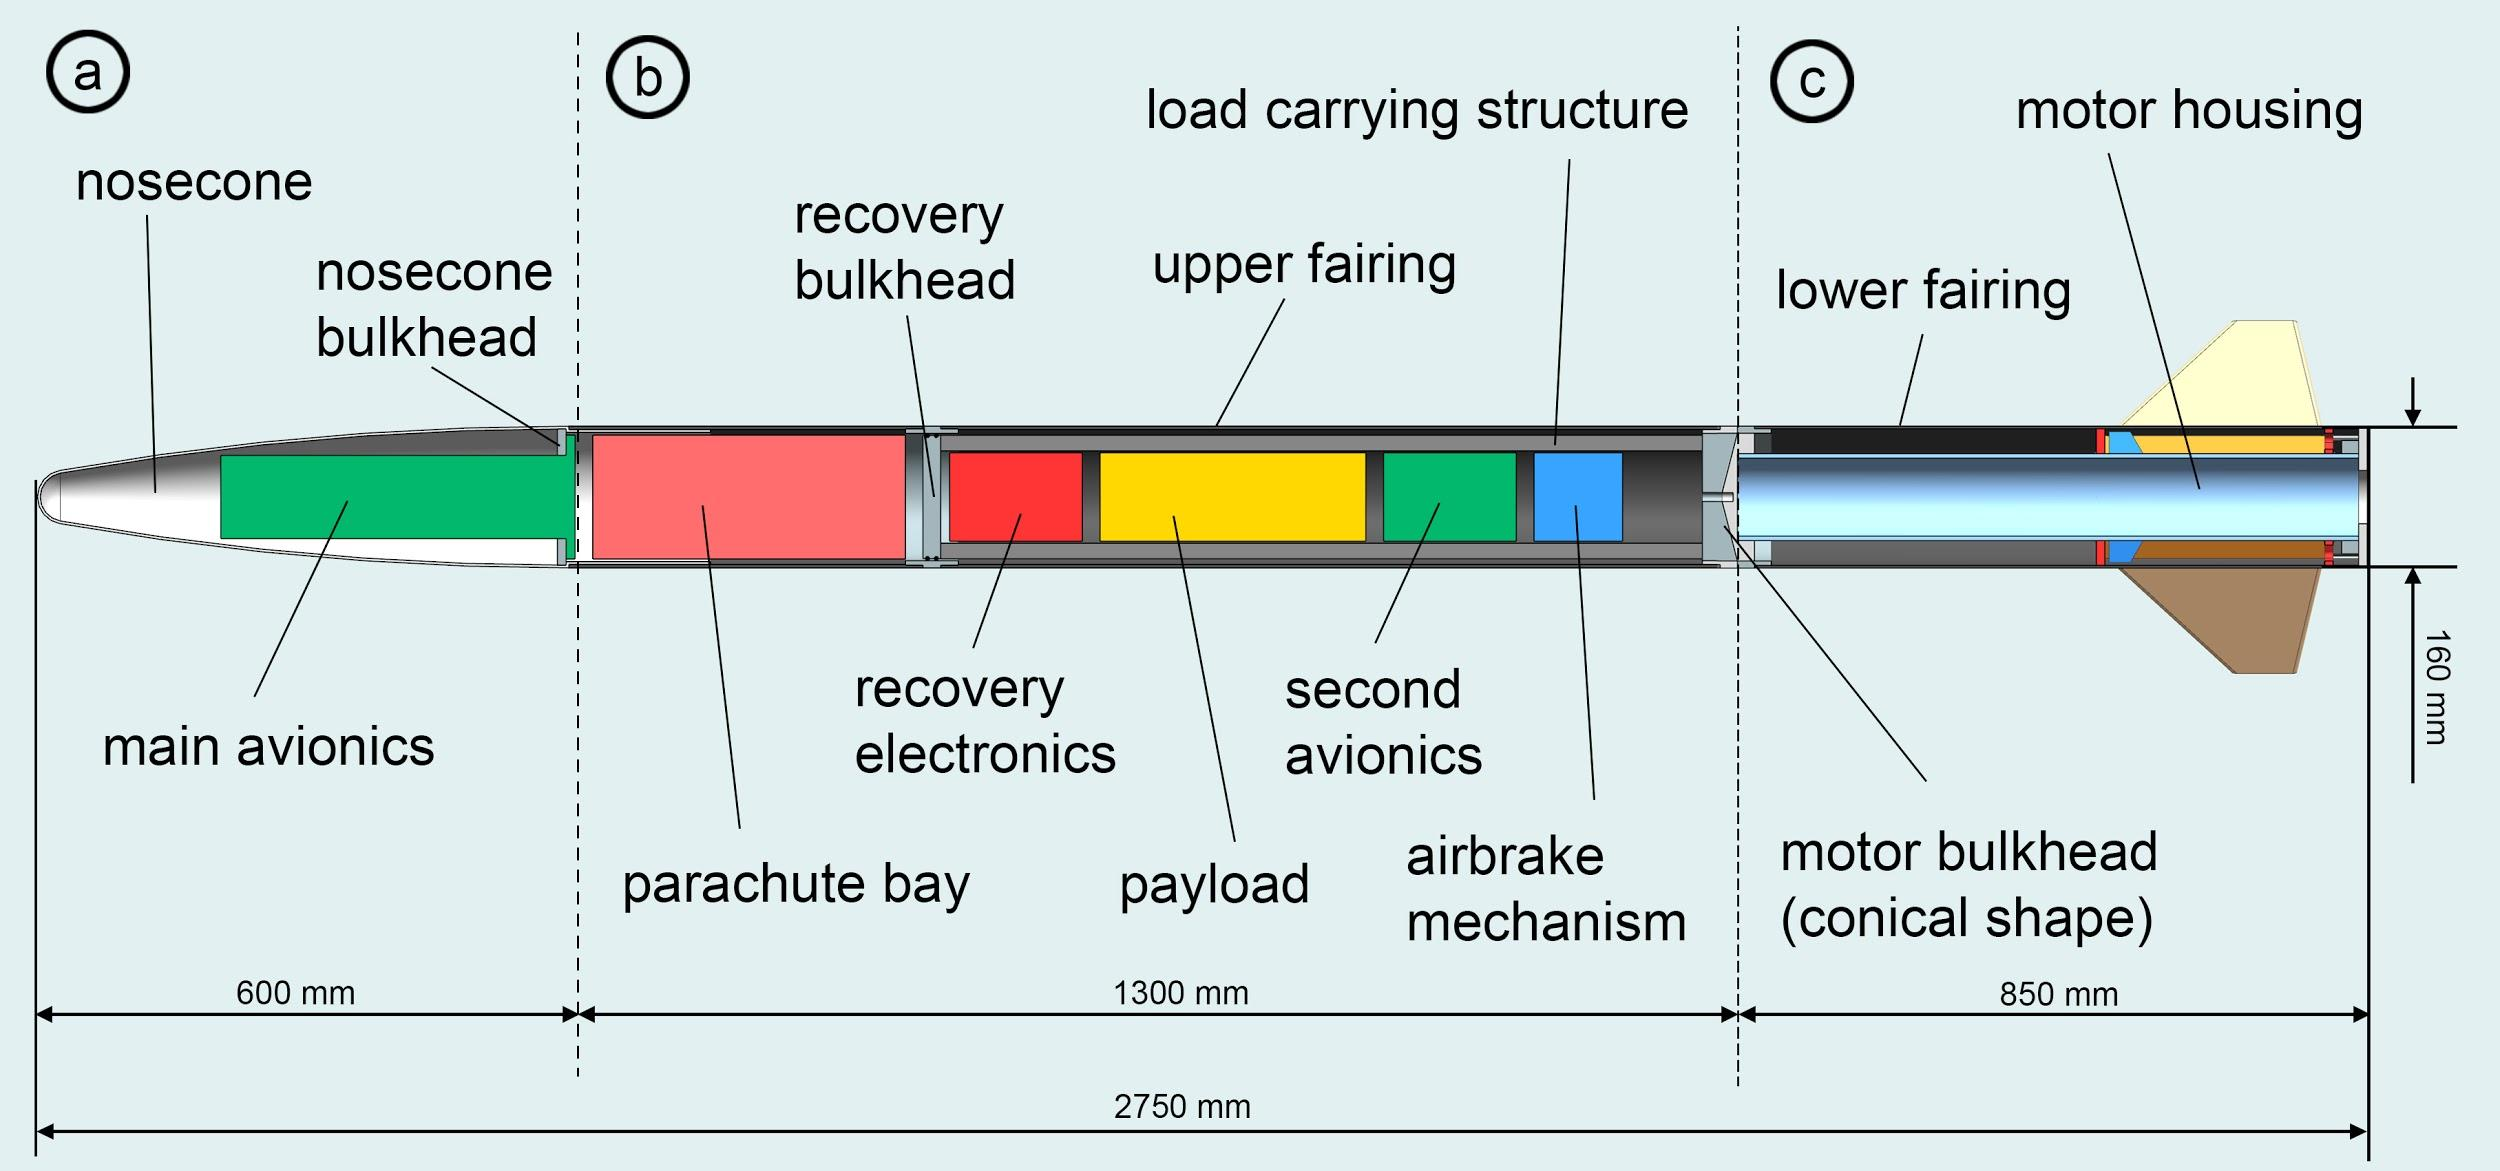
\includegraphics[width=.8\textwidth]{./Pictures/RocketModel.jpg}
 % RocketModel.jpg: 0x0 pixel, 300dpi, 0.00x0.00 cm, bb=
 \caption{Concept of the 2018 competition rocket Tell}
 \label{fig:2018RocketModel}
\end{figure}
 Figure \ref{fig:2018RocketModel} shows the rocket ``Tell'' which will be used in this year's competition.
 To aim for the right apogee a control algorithm is implemented on a micro controller that is placed in the lower body of the rocket.
 This control algorithm predicts the to-be-achieved apogee depending on the current states of the rocket (height, speed and acceleration).
 It then drives the air breaks to adjust that predicted apogee to the aimed 10 000 feet.
 This algorithm relays on the information of different sensors to determine the actual state of the rocket.
 Because there are different sensors to measure basically the same states, an algorithm which fuses this data to only one state information set would come in handy.
 With this fusion algorithm it should also be possible to be more accurate as with each sensor on its own.
 So the aim of this thesis is to implement a simulation for the sensor data provided during flight and with this simulation's help find the algorithm which is best suited for this task.\\
 For this the current situation of this year's project, the problem to be solved during this work and the desired solution will be described in this chapter.
 After that the models for the different sensors that will be used as well as the pros and cons of the different possible state estimators are discussed at the beginning of chapter \ref{ch:Approach}.
 In addition, different possible system models are also described in that chapter.
 Chapter \ref{ch:Implementation} will then show how the simulation and the fusion algorithm are implemented in detail.
 Furthermore will it discuss how the concepts that have been developed in the chapter before are integrated into the simulation.
 To verify that the implementation is working as intended, the results of the simulation and especially the performance of the different system models are discussed in chapter \ref{ch:Tests}.
 Finally, in the last chapter \ref{ch:Conclusion} a summary of the achieved knowledge, a comparison between the desired and the implemented solution and an outlook for coming work on this topic will be given.
 \newpage


 \section{Purpose}
 The hardware as well as the most of the software parts that will be used for this competition have already been defined.
 In addition it is a suitable assumption that the sensors and the dynamics of the rocket will stay more or less the same for the competitions coming.
 Therefore this thesis will focus mainly on finding an algorithm for this given surroundings, raise the performance at the competition flight itself and with this optimise the points achieved in the design implementation part.
 On top of that this thesis will also try to find an as modular solution as possible, so that the achieved knowledge can be reused and refined in further competitions.
 For this the dependencies and possibilities of the different sensors should be developed such that they can be fused in an optimal way.
 The final product should consist of a suitable fusion algorithm as well as a simulation part which provides the tools needed to test and adjust this fusion algorithm.

 \section{Research}
 Sensor data fusion and state estimation is a well established engineering field.
 Especially since the 1960 when Rudolf A. Kalman first published his paper about the Kalman filter.
 Those fusion algorithms are especially established in rocket science since they were first developed for the tracking of flying objects.
 Therefore there is already a lot of previous work which can be used in this thesis.
 Especially two books provided most of the needed theory. The first one of them is
 \cite{DavidWSchultz2004} which contains the basic theory about state estimation especially with Kalman filters. The second book
 \cite{SimonDan2006Ose:} is more focused on different approaches of state estimation and
 provides also different solutions to common problems that occur during the implementation of state estimations.
 In addition the Master Thesis \cite{BryanTongMinh2012} accesses more or less the same issue as this thesis does.
 Therefore in the conceptional part of this paper mainly this source will be used as a reference.

 \section{Sensors}
 \begin{figure}[h!]
  \centering
  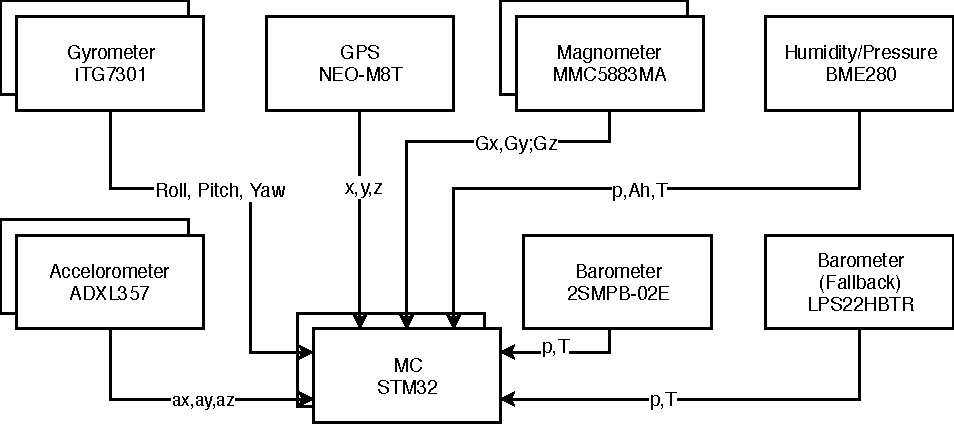
\includegraphics[width = \textwidth]{../BDADoku/Pictures/SensorNetworkAlt.pdf}
  \caption{Sensor Network}
  \label{fig:SensorNetwork}
 \end{figure}

 As mentioned above, different sensors are used in this year's competition to measure the current state of the rocket. Based on the assumption
 that basically the same sensors will be used in the coming competitions too, they will act as the basis for the sensor fusion algorithm.
 This used sensors and their settings will be described in this chapter.

 % Insert more information about those sensors if I get to them...
 \subsection{Accelerometer}
 First of all comes the accelerometer. Accelerometers are well established and widely used sensors which measure the force which is applied onto the sensor in the three space dimensions.
 This year's accelerometer is an ADXL357 which will be sampled at 1 000 Hz.

 \subsection{Gyrometer}
 The Gyrometer is needed to measure the rotational position of the Rocket. This is especially needed to determine if the rocket has a pitch angle. If so, the pure  acceleration on the z-axis can be calculated. The used gyrometer is ITG3701 and it will also be sampled at 1 000 Hz.

 \subsection{Barometers}
 Barometers are widely used in aviation because with a common pressure model the height can be easily calculated out of the measurements that the barometer takes.
 In this year's competition two barometers are used. These are by model name a 2SMPB-02E and a LPS22HBTR. They will be used with a sampling rate of 100 Hz each.
 In addition the humidity and pressure sensor BME280 can be used as an additional source for the pressure too.

 \subsection{Temperature}
 The temperature needs to be taken into account to make the height calculated out of the barometer data more accurate. This is because most of the atmospheric models depend besides of the pressure on the temperature as well.
 This temperature will be provided directly by the different barometers which each posses a separate temperature sensor.

 \subsection{Magnometer}
 Also there are two Magnometers in the sensor network. They measure the strength of the surrounding magentic field.
 This can be used to determine the direction in relation to the north pole.
 Due to the fact that the algorithm that will be developed in this thesis does not include the x- and y-axis in its calculations,
 this sensor will not be used for the sensor fusion algorithm.

 \subsection{GPS}
 For the next year's competition a differential GPS should be in place as well with the help of two $\mu$block modules.
 This measurements are more precise as the rest of the sensors but are taken at a much slower sample rate around 0.5 - 2Hz.
 Therefore the algorithm should already take these measurements into account too and interpolate them with the data from the other sensors.

 \section{Problems}
 Out of the research and the previous competitions, different problems appeared that need to be addressed in this thesis to ensure an as good as possible solution.

 \subsection{Different Sensors}
 First of all there are different sensors which all do measure different values and have different parameters (precision, sampling time).
 So the algorithm has to extract the strengths out of the different sensors and minimise their individual weaknesses.
 Additionally because this algorithm is system critical, it has to be reliable enough that it still works properly if any of the sensors are failing.

 \subsection{System Load}
 The cycling time will be around 1 ms on the embedded system. This time was chosen on behalf that it would be difficult to get the precisely needed cycling time to ensure the needed controllability of the rockets apogee.
 Therefore the system load that the algorithm will cause has to be strongly limited for it to be able to run on this given system.
 The system this year is a 32 bit ARM SoC which runs at 168 MHz. Assumed that the whole control software has at maximum half of a software cycle at his disposal the maximum clock cycles to be used for all calculations in one such software cycle is around 84 000.
 With this amount of cycles the processor can do around 10 000 simple calculations (addition, subtraction, multiplication or division),
 because its floating point unit needs on average around 8.5 cycles per operation (load, calculate and store). Of these 10 000 simple calculations at most 5 000 may be used by the sensor fusion algorithm.
 This number is just a rough assumption, which means that the final system load should aim to not reach this value or at least not exceed it by a great number.

 \subsection{Precision}
 The precision is after the system load the most critical attribute. If the algorithm fails to provide the required accuracy the control algorithm has no exact height estimation to rely on.
 The control requirements state that the maximum error between the estimated and the real height should not exceed two meters to be able to properly control the aim of the apogee.
 This accuracy is especially needed after the burnout when the apogee control with the air brakes will start.

 \subsection{Settling Time}
 The settling time is defined as the time span between the first reliable measurement after the burnout and the time  the estimation reaches its required precision.
 This time span has to be small enough to ensure that the control has enough time to aim for the desired apogee. In the current system the burnout occurs around 3-3.5 seconds after ignition while the whole flight upwards only takes around 25 seconds. Therefore the settling should be finished at most
 one second after burnout so that the control has as much time as possible for the aiming. Best would be if the algorithm already achieves its target precision while the motor is still burning.

 \subsection{Reliability}
 Due to how a sensor package is placed into the rocket, the assumption has to be made that it will be possible that sensors fail in execution.
 Therefore the algorithm should be reliable enough to still provide the control system with the desired data with some of the sensors failed, so the functionality of the whole system reamins intact. But of course the provided data has not to be as accurate any more as it would be with all sensors working.

 \subsection{Modularity}
 Although it can be assumed that the sensors will stay more or less the same over the next competitions, it is not certain that exactly the same sensors will be used.
 Therefore the presented algorithm should provide the possibility to adapt to new sensors in an easy way, as long as they resemble the old sensor in a feasible way.
 This will ensure a long term usability of the provided algorithm.

 \section{Requirements}

 \begin{table}[h]
 \centering
 \begin{tabular}{|l|l|l|l|}
 \hline
 \bf{Requirement}   & \bf{Rating} & \bf{Aim} & \bf{Importance} \\ \hline
 System Load   & \# Calculation steps per loop & < 5000 & Critical \\ \hline
 Precision     & Error between estimation and ground truth  & < 2 m in height & High  \\ \hline
 Settling Time & Time from first reliable to optimal estimation  & < 1 s after burnout &  High \\ \hline
 Reliability   & Working estimation with \# failed sensors & 2-3 sensors & Medium \\ \hline
 Modularity    & Effort needed to change a sensors & < 10 h work &  Desirable \\ \hline
 \end{tabular}
 \caption{Requirements table}
 \label{tab:Requirements}
 \end{table}

 As seen in the table \ref{tab:Requirements} five requirements were drown out of the problem analysis.
 First of all there is one critical requirement, namely the system load. This one is given the importance ``critical'' because the algorithm needs to be efficient enough to run on the embedded system given.
 Any solution that would exceed the value given in this requirement in a great manner would be pointless in the frame of this thesis, because it will not be deployable to the target system.

 Secondly there are two requirements which are tied together, the precision and the settling time.
 Where the precision describes what an optimal estimation is in regard to the scope of this thesis, the settling time relies on this precision beeing reached as soon as possible.
 The settling time is defined as the time span between the burnout until the best possible precision is achieved.

 The modularity as well as the reliability requirements are more guidelines than hard requirements.
 This because they will still lead to a usable solution for this year's project and their aim is hard to define since it is depending on the coming competitions and their circumstances.

 \section{Desired Solution}
 The desired solution should meet all of the given requirements as good as possible.
 While doing this it should also not get more complicated than needed because an easy understandable solution helps to ensure its further use in coming competitions.
